\documentclass[11pt,a4paper]{article}

% --- Core packages ---------------------------------------------------------
\usepackage[utf8]{inputenc}
\usepackage[T1]{fontenc}
\usepackage{lmodern}
\usepackage{microtype}
\usepackage[margin=1in]{geometry}
\usepackage{graphicx}
\usepackage{booktabs}
\usepackage{caption}
\usepackage{subcaption}
\usepackage{amsmath,amssymb}
\usepackage{xcolor}
\usepackage{listings}
\usepackage{hyperref}
\usepackage{titlesec}
\usepackage{enumitem}
\usepackage{fancyhdr}

% --- Colours & links -------------------------------------------------------
\definecolor{nusblue}{HTML}{003D7C}
\definecolor{accent}{HTML}{E08A1F}
\definecolor{inkcolor}{HTML}{10182C}
\definecolor{mutedcolor}{HTML}{5B5F6B}
\definecolor{codebg}{HTML}{F3EEE2}

\hypersetup{
  colorlinks=true,
  linkcolor=nusblue,
  urlcolor=nusblue,
  citecolor=nusblue,
}

% --- Section styling -------------------------------------------------------
\titleformat{\section}{\color{nusblue}\large\bfseries}{\thesection}{0.7em}{}
\titleformat{\subsection}{\color{inkcolor}\normalsize\bfseries}{\thesubsection}{0.6em}{}

% --- Header / footer -------------------------------------------------------
\pagestyle{fancy}
\fancyhf{}
\renewcommand{\headrulewidth}{0.3pt}
\fancyhead[L]{\small\color{mutedcolor}NUS CS5260 -- Final Project}
\fancyhead[R]{\small\color{mutedcolor}PyCallingAgent}
\fancyfoot[C]{\small\color{mutedcolor}\thepage}

% --- Listings --------------------------------------------------------------
\lstdefinestyle{py}{
  language=Python,
  basicstyle=\ttfamily\footnotesize,
  keywordstyle=\color{nusblue}\bfseries,
  stringstyle=\color{accent!80!black},
  commentstyle=\color{mutedcolor}\itshape,
  numberstyle=\tiny\color{mutedcolor},
  backgroundcolor=\color{codebg!50},
  frame=single,
  rulecolor=\color{mutedcolor!40},
  breaklines=true,
  showstringspaces=false,
  captionpos=b,
}
\lstset{style=py}

% --- Title -----------------------------------------------------------------
\title{%
  \vspace{-2em}
  \color{accent}\large NUS CS5260 \textendash{} Final Project Report\\[0.6em]
  \color{inkcolor}\Huge\bfseries PyCallingAgent\\[0.3em]
  \color{inkcolor}\large\mdseries A Prompt-First Financial Research Agent\\[-0.2em]
  \color{inkcolor}\large\mdseries Built on a Stateful Python Runtime
}

\author{%
  Zhenglin Wan \quad\textbar\quad Tianhao Yao\\
  \small National University of Singapore\\
  \small \texttt{vanzl@u.nus.edu}
}

\date{\small April 2026}

% ============================================================================
\begin{document}
\maketitle
\thispagestyle{fancy}

\begin{center}
\begin{minipage}{0.92\linewidth}
\centering
\color{mutedcolor}\small
\textbf{Live demo:} \href{https://pycallingagent.onrender.com}{\texttt{pycallingagent.onrender.com}} \quad\textbar\quad
\textbf{Source:} \href{https://github.com/vanzll/PyAgent}{\texttt{github.com/vanzll/PyAgent}}\\[0.4em]
\textit{\small The live demo is hosted on a free tier. If the page does not load, the instance may have fallen asleep due to inactivity -- please contact the author (\href{mailto:vanzl@u.nus.edu}{vanzl@u.nus.edu}) so we can re-activate it on the hosting platform.}\\[0.3em]
\textit{For research and coursework demonstration only. Not investment advice.}
\end{minipage}
\end{center}
\vspace{0.6em}

% --- Abstract --------------------------------------------------------------
\noindent\textbf{\color{nusblue}Abstract.}\quad
LLM-based agents typically interact with tools through JSON function calling, which forces every object to be serialised into text between calls. For data-intensive research tasks, this paradigm is inefficient: DataFrames are flattened into strings, complex objects cannot persist across turns, and the model cannot cheaply compose in-memory results. \textbf{PyCallingAgent} is a prompt-first financial research agent built on a persistent Python runtime that removes this text bottleneck. The system pairs a lightweight \textit{semantic track} (the LLM message history) with a long-lived \textit{runtime track} (an IPython kernel), so that rich objects such as market DataFrames and analytic helpers live inside the runtime across turns, while only compact descriptors enter the prompt. On top of this runtime, we build a financial research pipeline that fetches grounded data from SEC EDGAR and public market sources, injects it as live variables, and lets the agent produce both a language answer and visible work products (charts, tables, downloadable reports) within a single turn. The product is deployed as a FastAPI web service at \href{https://pycallingagent.onrender.com}{\texttt{pycallingagent.onrender.com}} and demonstrates how a research-grade agent runtime can be packaged as an end-user product.

\medskip
\noindent\textbf{\color{nusblue}Keywords:}\quad LLM agents, stateful runtime, tool calling, agent skills, financial research, FastAPI.

\vspace{0.6em}
\hrule height 0.5pt
\vspace{1em}

% ============================================================================
\section{Introduction}

Large language model agents are increasingly used as the glue between natural-language instructions and external tools. The dominant pattern is \emph{JSON function calling}: the model emits a tool name and a JSON argument blob; the runtime executes the call; the return value is serialised into a string and appended back into the prompt. This pattern is effective for simple, stateless tools such as a weather lookup or a calculator, but three limitations become visible once the workload is more data-intensive:

\begin{itemize}[leftmargin=1.3em,itemsep=0.2em]
    \item \textbf{Serialisation tax.} Any non-trivial object (a DataFrame, a fitted model, a chart, a database cursor) must be flattened into text before the agent can reason about it again. A thousand-row table ends up consuming thousands of prompt tokens for a single turn.
    \item \textbf{Lack of persistent state.} Tool calls are stateless. A variable produced on turn $t$ cannot be reused on turn $t{+}1$ without being either re-serialised into the prompt or re-computed from scratch.
    \item \textbf{Weak composition.} Because all intermediate values are strings, the model cannot chain them with a couple of lines of code. It ends up \emph{re-describing} data rather than \emph{computing} on it.
\end{itemize}

For financial research -- which is inherently data-heavy -- these limitations are crippling. The agent spends its context window paraphrasing numbers it has already pulled, and it cannot easily re-use intermediate DataFrames across follow-up questions.

This report presents \textbf{PyCallingAgent}, a prompt-first financial research agent that addresses these limitations by elevating a persistent Python runtime to be the central workspace. Instead of treating the LLM's context window as the source of truth, we treat a long-lived IPython kernel as the source of truth and let the LLM generate short snippets of Python that operate on it. The LLM's prompt only needs to carry a catalogue of available objects and functions, not their full contents.

PyCallingAgent is implemented as an NUS CS5260 final project. The system is organised as two layers: a persistent-runtime and skills infrastructure that sits underneath, and a financial research product layer built on top -- including the data pipeline, the FastAPI web application, the session and run orchestration, and the deployed public instance.

\paragraph{Contributions.} This report contributes:
\begin{enumerate}[leftmargin=1.3em,itemsep=0.2em]
    \item a design writeup of how a stateful-runtime agent can be wrapped into a deployable web product for financial research;
    \item a working implementation, publicly deployed at \href{https://pycallingagent.onrender.com}{\texttt{pycallingagent.onrender.com}}, that accepts natural-language prompts and returns grounded research artefacts (charts, tables, reports);
    \item a discussion of the application-layer adaptations (FastAPI, session/run orchestration, SSE-style progress streaming, graceful fallback under API rate limits) that were required to turn a stateful agent loop into a robust web service.
\end{enumerate}

% ============================================================================
\section{Background and Related Work}

\paragraph{From text I/O to code-as-action.}
Early LLM agents treated the model as a pure text-in/text-out generator and composed tool use through prompt templates such as ReAct-style thought/action traces. JSON function calling formalised this by defining a structured schema for tool arguments. A later line of work replaces JSON with small snippets of \emph{code} that the model writes and the runtime executes -- often referred to as \emph{code-as-action}. This lets the model compose operations more naturally (loops, conditionals, arithmetic) but, crucially, most such systems still execute each snippet in an ephemeral sandbox and return the output as a string. State does not persist between calls.

\paragraph{Stateful runtimes.}
More recent proposals move toward a stateful Python runtime that is kept alive across agent turns. Variables defined on one turn remain accessible on the next; complex objects can be held in the runtime without being materialised back into the prompt. PyCallingAgent follows this line of work: it includes a persistent IPython runtime, an injection API for variables and functions, and an Agent Skills-compatible loader. In this report we describe these components briefly and focus on the product layer and its application-level adaptation.

\paragraph{Agent Skills.}
The Agent Skills standard specifies how reusable skill packages can be bundled (as a directory with an instruction file and optional executable extensions) and discovered by agents at runtime. Our financial research pipeline is packaged as a set of such skills (e.g. \texttt{fundamentals}, \texttt{market-data}, \texttt{financial-comparison}, \texttt{charting}, \texttt{report-writer}), each of which can inject Python callables directly into the runtime at activation time.

% ============================================================================
\section{System Design}

\subsection{Overview: Semantic Track and Runtime Track}

The agent maintains two parallel but synchronised tracks throughout an interaction. A \emph{semantic track} carries the LLM message history forward one step per turn, while a \emph{runtime track} keeps a long-lived IPython kernel alive whose state persists across turns and holds DataFrames, functions, and other Python objects. Only compact observations are folded from the runtime back into the semantic track, keeping the prompt small while the workspace grows.

Formally, the semantic track updates according to
\begin{equation}
    h_t = \mathrm{LLM}(x_t,\, h_{t-1}),
\end{equation}
where $h_t$ is the conversational history after step $t$ and $x_t$ is the new input. The runtime track updates according to
\begin{equation}
    s_t = \mathrm{exec}(c_t,\, s_{t-1}),
\end{equation}
where $c_t$ is the code block emitted by the LLM at step $t$ and $s_t$ is the state of the Python kernel. The two tracks interact through a bounded \emph{observation function} $\tau(s_t)$ that returns a compact summary (shapes, column names, head rows, print-ed outputs truncated to a length budget) to be folded back into $h_t$. Full objects never enter $h_t$.

The practical consequence is that the prompt remains small and bounded, while the workspace capacity is effectively the runtime's memory rather than the context window.

\subsection{Runtime Primitives}

The runtime exposes three injection primitives:

\begin{itemize}[leftmargin=1.3em,itemsep=0.2em]
    \item \textbf{Variable} -- any Python object, registered under a name. The LLM only sees the name and a short description; it retrieves the object by writing normal Python.
    \item \textbf{Function} -- a Python callable, surfaced to the LLM along with its docstring and signature.
    \item \textbf{Type} -- a class or dataclass; a schema is auto-extracted (Pydantic, dataclasses, and Enums are supported) so the LLM can construct well-typed instances.
\end{itemize}

A minimal usage sketch is shown in Listing~\ref{lst:inject}.

\begin{lstlisting}[caption={Injecting a DataFrame and a function into the runtime.},label={lst:inject}]
from pycallingagent import PyCallingAgent, Variable, Function
from pycallingagent.runtime import IPythonRuntime
from pycallingagent.models import LiteLLMModel

runtime = IPythonRuntime(
    variables=[Variable("prices", price_df, "Daily OHLCV for AAPL")],
    functions=[Function(fetch_fundamentals)],
)
agent = PyCallingAgent(model=model, runtime=runtime)
await agent.run("Compare AAPL and NVDA on valuation.")
\end{lstlisting}

\subsection{Skills with Progressive Disclosure}

To avoid bloating the prompt with every possible capability, skills are loaded in two stages (Figure~\ref{fig:skills}):

\begin{enumerate}[leftmargin=1.3em,itemsep=0.2em]
    \item \textbf{At startup}, only metadata (name and one-line description) is placed in the system prompt -- roughly 100 tokens per skill.
    \item \textbf{On demand}, when the agent calls the built-in \texttt{activate\_skill(name)}, the full instruction body is appended to the prompt and any callables exported by the skill's \texttt{injection.py} are injected into the runtime.
\end{enumerate}

This is a variant of progressive disclosure: the prompt carries a table of contents, while the full library lives in the runtime. Empirically, this lets us ship a meaningful skill catalogue without paying its cost on turns that do not need it.

\begin{figure}[t]
    \centering
    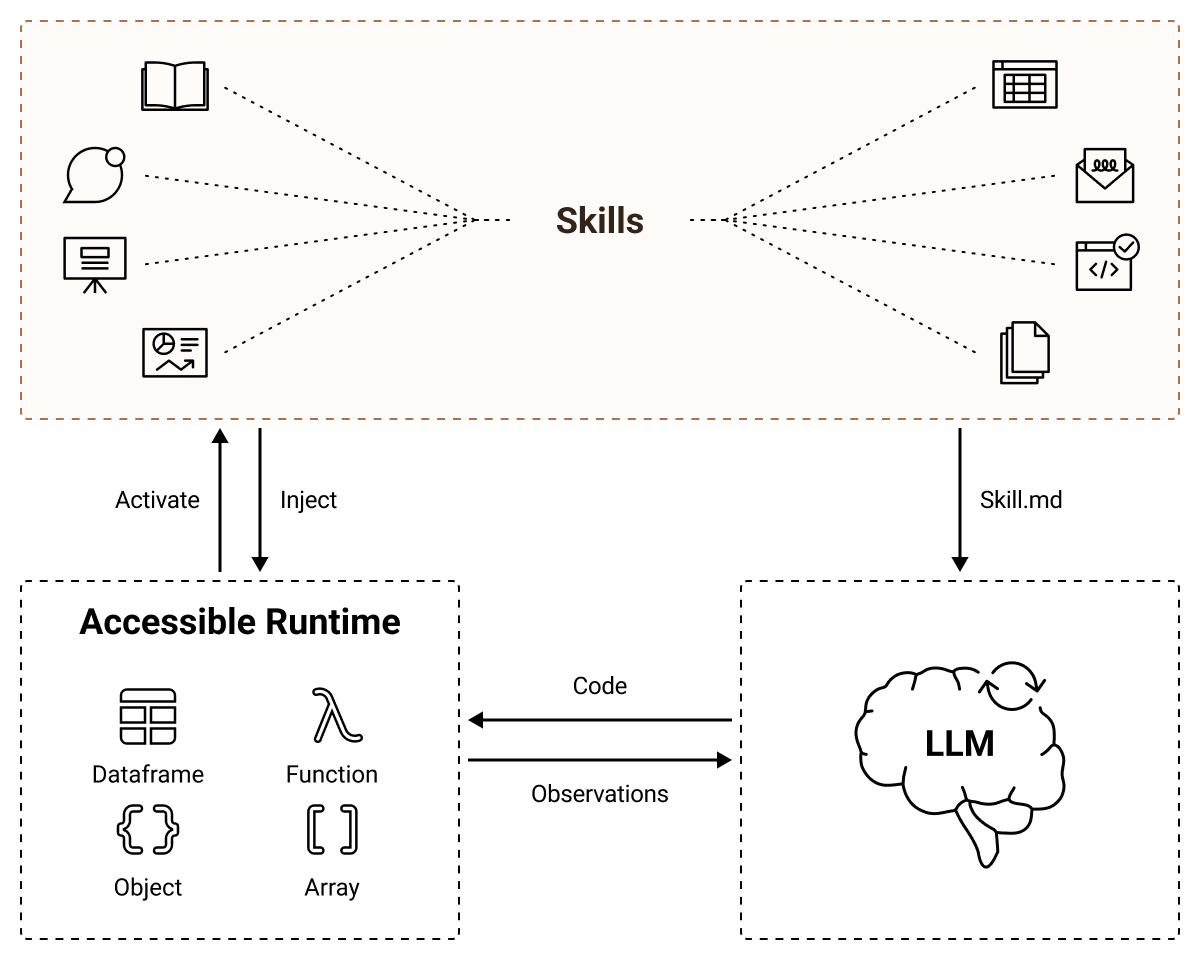
\includegraphics[width=0.8\linewidth]{figures/Skills.png}
    \caption{Skill system. Skills are directories with a markdown instruction file and an optional \texttt{injection.py} that exports Python callables. On activation, both the instructions and the callables are injected into the agent's accessible runtime.}
    \label{fig:skills}
\end{figure}

\subsection{AST-Based Security}

Because the LLM can generate arbitrary Python, every code block is first parsed and validated at the AST level before being dispatched to the kernel. Four rule types are supported: \texttt{ImportRule} (allow/deny specific modules), \texttt{FunctionRule} (forbid dangerous calls such as \texttt{eval} or \texttt{exec}), \texttt{AttributeRule} (restrict dunder access), and \texttt{RegexRule} (catch residual patterns). Violations never reach the kernel; the agent receives a structured error instead and can regenerate the code.

% ============================================================================
\section{Financial Research Pipeline}

The financial research product layer is a thin orchestrator on top of the runtime. One user prompt triggers a five-step pipeline:

\begin{enumerate}[leftmargin=1.3em,itemsep=0.2em]
    \item \textbf{Parse.} We classify the prompt as finance-related or generic. Finance prompts are analysed to extract candidate tickers (e.g. \texttt{AAPL}, \texttt{NVDA}) or market proxies (e.g. \texttt{SPY}). Generic prompts fall through to a chat-only path so that small talk does not error.
    \item \textbf{Fetch grounded data.} We query SEC EDGAR for fundamentals, optionally Alpha Vantage for market data, and use a stable public-data fallback when third-party APIs are unavailable or rate-limited.
    \item \textbf{Inject into the runtime.} Price DataFrames, fundamentals, and a small library of helper functions are registered as \texttt{Variable}s and \texttt{Function}s in the kernel. The LLM's prompt only sees their descriptors, not their contents.
    \item \textbf{Run the agent.} The agent selects and activates relevant skills, writes Python that operates on the injected objects, and produces charts, tables, and a textual summary.
    \item \textbf{Materialise outputs.} Artefacts (PNG charts, CSV/XLSX tables, a markdown report) are written to the session's working directory, previewed in the web UI, and made downloadable.
\end{enumerate}

A single turn therefore yields both a natural-language answer and visible work products, which is why the user experience feels more like an analyst assistant than a dashboard.

% ============================================================================
\section{Application-Layer Adaptation}

Wrapping a stateful agent loop inside a stateless HTTP request model was the most non-trivial engineering work in the project. The deployed application is a FastAPI service with a Jinja2-plus-vanilla-JS frontend, structured around three main pieces of glue.

\subsection{Session and Run Orchestration}

Each \emph{session} owns a persistent IPython kernel and a working folder. Within a session, each user prompt becomes a \emph{run}, which owns an event log and a set of artefacts. Runs are cancellable (so the user can interrupt a slow analysis) without killing the kernel, so follow-up prompts remain fast because the runtime state is preserved. The contract we settled on -- \emph{session owns the kernel, run owns the work, events are append-only} -- turned out to be the simplest one that survives network flakiness and user cancellation.

\subsection{Progress Streaming}

We push progress events to the browser over a Server-Sent-Events stream, with a polling fallback for networks that cannot keep a long-lived connection open. The frontend renders the latest events as a sliding-window ``Live Status'' panel, so the user sees the pipeline move through its stages (fetching data, running agent, materialising outputs) rather than staring at a spinner.

\subsection{Artefact Rendering}

Every artefact written during a run is registered in the session. Tables are previewed in-page using the first ten rows; charts are previewed as inline PNGs; the markdown report is rendered directly in the browser. Full files are also exposed as download endpoints so the user can open them offline. The combination of inline preview plus download keeps the page useful both during a live demo and as a static reference afterwards.

% ============================================================================
\section{Deployment}

The deployed instance runs on Render, using the \texttt{render.yaml} blueprint in the repository. The deployment surface is deliberately minimal:

\begin{itemize}[leftmargin=1.3em,itemsep=0.2em]
    \item \textbf{Build}: \texttt{pip install '.[openai,webapp]'}.
    \item \textbf{Start}: a single \texttt{uvicorn} command launching the FastAPI application factory.
    \item \textbf{Config}: a small set of environment variables -- \texttt{LLM\_MODEL\_ID}, \texttt{LLM\_API\_KEY}, \texttt{LLM\_BASE\_URL}, \texttt{SEC\_USER\_AGENT}, and an optional \texttt{ALPHAVANTAGE\_API\_KEY}.
\end{itemize}

One choice worth calling out is the \textbf{public-data mode}: the product keeps working even when no Alpha Vantage key is configured, by combining SEC filings with a stable public market-data fallback. This was essential for a classroom setting because free-tier market APIs regularly rate-limit and would otherwise make the demo unreliable during a talk.

The deployed URL is \href{https://pycallingagent.onrender.com}{\texttt{pycallingagent.onrender.com}}.

% ============================================================================
\section{Qualitative Demonstration}

We use two prompts as canonical demos.

\paragraph{Demo A: single-ticker summary.}
Prompt: \emph{``Summarize Apple and show the recent price trend.''}
The system infers \texttt{AAPL}, fetches price history and a small fundamentals snapshot, and returns a three-paragraph summary together with a trend chart, a table of key metrics, and a downloadable markdown report. The chart is computed from the DataFrame in the runtime, not narrated from the model's parametric memory.

\paragraph{Demo B: cross-ticker comparison.}
Prompt: \emph{``Compare AMD and Nvidia on valuation and performance.''}
The system extracts both tickers, loads data for each, and produces a side-by-side comparison table (valuation multiples, year-on-year metrics), a dual-series chart overlaying both tickers' price trajectories, and a short comparative brief. Because both tickers' DataFrames live in the runtime simultaneously, the comparison can be expressed in a few lines of Python rather than in a long textual paraphrase.

\paragraph{Persistence across follow-ups.}
Because the runtime state survives across turns, follow-up prompts are cheap. If the user first asks ``compare AMD and Nvidia on valuation'' and then follows up with ``now also show their 5-year revenue CAGR'', the DataFrames loaded during the first turn are still in the kernel and can be reused by the second turn without re-fetching or re-serialising. The same mechanism supports richer interactive analyses such as refining a chart, adjusting a time window, or drilling into a specific metric within the same session.

% ============================================================================
\section{Discussion and Limitations}

\subsection{What the Project Demonstrates}

PyCallingAgent shows that a research-flavoured agent runtime (persistent kernel, injection API, progressive-disclosure skills) can be wrapped into a deployable web product without fighting its abstractions. The hard parts were not in the runtime; they were in the \emph{contract} between the stateful kernel and the stateless web layer. Once the session/run/event model was chosen, the rest of the product layer -- streaming, artefact rendering, cancellation -- fell out of it naturally.

\subsection{Limitations}

\begin{itemize}[leftmargin=1.3em,itemsep=0.2em]
    \item \textbf{Python-centric.} Any skill we want to ship has to be expressible as Python. This rules out non-Python tools unless they are wrapped.
    \item \textbf{Free-tier API fragility.} Alpha Vantage and similar free endpoints rate-limit aggressively; public-data mode mitigates but does not eliminate this.
    \item \textbf{LLM-written prose.} Numbers are grounded in runtime data, but the natural-language summary is still written by the LLM. We frame the product as research assistance rather than certified financial reporting.
    \item \textbf{No quantitative evaluation.} This report is qualitative; a formal benchmark of task-completion rate or user preference is out of scope for a course project but would be a natural next step.
\end{itemize}

\subsection{Future Work}

Natural extensions include: richer multi-agent coordination over a shared runtime (so a ``data agent'' and a ``writing agent'' can exchange objects instead of text), better memory-management policies for very long-running sessions, and a programmatically-scored benchmark harness that uses the runtime state to verify agent outputs automatically (the runtime is inspectable, which is what made this feasible in principle).

% ============================================================================
\section{Conclusion}

We presented PyCallingAgent, a prompt-first financial research agent built on a persistent Python runtime. By separating a lightweight semantic track from a long-lived runtime track, the system keeps the LLM's prompt small while letting rich objects -- DataFrames, fitted helpers, intermediate results -- persist across turns. On top of this runtime, we built a financial research pipeline that grounds outputs in SEC and public market data, and wrapped it in a FastAPI web product with session/run orchestration, streamed progress, and inline artefact rendering. The deployed instance at \href{https://pycallingagent.onrender.com}{\texttt{pycallingagent.onrender.com}} serves as a working demonstration that a stateful-runtime agent paradigm can be delivered as an end-user product within the scope of a single-semester course project.

% ============================================================================
\section*{Acknowledgements}

This project was completed as the final submission for NUS CS5260. We thank the course instructors and teaching assistants for their guidance. SEC EDGAR is used as the primary public data source for U.S.\ company filings, and the public instance is hosted on Render's free tier.

\bigskip
\noindent\fbox{\begin{minipage}{0.97\linewidth}
\footnotesize
\textbf{Live demo}: \href{https://pycallingagent.onrender.com}{\texttt{https://pycallingagent.onrender.com}}\\
\textbf{Source}: \href{https://github.com/vanzll/PyAgent}{\texttt{https://github.com/vanzll/PyAgent}}\\
\textbf{License}: MIT.\quad \textbf{Disclaimer}: research and coursework demonstration; not investment advice.
\end{minipage}}

\end{document}
